


En este apartado, se presenta un tipo de relación entre conjuntos muy
empleado en todas las áreas matemáticas.

Definición. Aplicación entre conjuntos. Una relación $F$ entre los conjuntos
$A$ y $B$, $F \subseteq A \times B$, se denomina \emph{aplicación}
(\emph{mapping}) o \emph{función} (\emph{function}) entre $A$ y $B$ si y
solo si todos y cada uno de los elementos del conjunto inicial $A$ de la
relación se encuentran relacionados con un único elemento del conjunto final
$B$.

Es decir, una aplicación $F$ del conjunto $A$ al conjunto $B$ es un
subconjunto $F \subseteq A \times B$ tal que, para todo $x \in A$, se tiene
que el conjunto imagen de este, $F(x)$, es un conjunto unitario.

Si prefiere una definición más simbólica: $F: A \longrightarrow B$ es
aplicación si y solo si:

$$ \forall x \in A,\ \exists! y \in B \st F(x) = \{y\} $$

Ya que ese conjunto imagen de $x$ consta de un solo elemento, se suele
prescindir de las llaves en la representación de este. Así, se suele
escribir $F(x) = y$, en lugar de $F(x) = \{y\}$. Indistintamente, se
utilizan letras mayúsculas o minúsculas al referirnos a una aplicación. La
terminología usualmente empleada para la aplicación

$$ f: A \longrightarrow B $$

\noindent es la siguiente.

Al conjunto $A$ se le suele llamar es el \emph{dominio de definición}, o,
simplemente, \emph{dominio} (\emph{domain}), cosa que denotamos por
`$\text{Dom}(f)$' o `$\text{Dom}\ f$'. También, puede recibir los nombres
que le dimos en las relaciones: \emph{conjunto inicial}, \emph{conjunto
original}, etc., y se ven representaciones como `$\text{Orig}(f)$' y
`$\text{Orig}\ f$'.

El conjunto $B$ es el \emph{codominio} (\emph{codomain}). También, puede ver
que lo llaman \emph{conjunto final}, como se hacía en las relaciones.

El conjunto

$$ f(A) = \{y \in B \st \exists x \in A.\ f(x) = y\} = \{f(x) \st x \in A\}
$$

\noindent se denomina \emph{conjunto imagen} de la función, `$\text{Im}(f)$'
o `$\text{Im}\ f$'. También, \emph{recorrido} o \emph{rango} (\emph{range}).

El elemento $f(x)$ se denomina \emph{imagen} del elemento $x$ o simplemente
\emph{imagen} de $x$.

El conjunto original del elemento $y \in B$ mediante la aplicación $f$, o
simplemente \emph{original} de $y$, se representa como

$$ f^{-1}(y) = \{x \in A \st f(x) = y\} $$

\noindent y se denomina \emph{imagen inversa} de $y$ o \emph{contraimagen}
de $y$.

El conjunto de todas las aplicaciones de $A$ a $B$ se denota por
`$\mathcal{F}(A, B)$' o `$B^{A}$'. Para el caso de que $A = B$, se pone
`$\mathcal{F}(A)$'.

Observaciones.

Dada una aplicación $f: A \longrightarrow B$, si el conjunto $A$ es el
conjunto vacío, $A = \emptyset$, entonces, como sabemos de las relaciones,
el producto cartesiano $A \times B$ será también el conjunto vacío, $A
\times B = \emptyset$. De dicho conjunto solo existe un subconunto;
concretamente, $\emptyset$. Por tanto, esa será la única relación que se
puede dar en este caso, $\emptyset \subseteq \emptyset \times B$, y, si se
fija, esta relación cumple las condiciones para ser considerada una
aplicación, $f: \emptyset \longrightarrow B$, ya que se puede decir que,
para este caso, esas condiciones son vacuamente ciertas. Se la suele llamar
\emph{aplicación vacía}.

Sin embargo, si se tiene $A \neq \emptyset$ y $B = \emptyset$, el producto
cartesiano $A \times B$ es también el conjunto vacío, $A \times B =
\emptyset$, y, al igual que antes, solo existe un subconjunto de este: el
conjunto vacío, $\emptyset$. Dicho conjunto será una relación. La diferencia
con el caso anterior está en que esta relación no es una aplicación ya que
existirán elementos del conjunto original $A$ que no tienen imagen, cosa que
incumple una de las condiciones para ser una aplicación.

En resumen, se tiene que $\mathcal{F}(\emptyset, B) = \{\text{aplicación
vacía}\}$ mientras que $\mathcal{F}(A, \emptyset) = \emptyset$ si $A \neq
\emptyset$.

Aunque el significado de los términos \emph{función} y \emph{aplicación} es
el mismo, estos términos no suelen usarse indistintamente. El término
\emph{función} se aplica, en general, cuando el conjunto final es un
conjunto de números ($B \subset \rset, B \subset \cset, \ldots$) o un
conjunto producto de conjuntos numéricos ($B \subset \rset^n, B \subset
\cset^n, \ldots$). Esto no es una regla estricta, pues de hecho se
encuentran con frecuencia expresiones del tipo ``La función $f : \rset^2 \to
\rset$ definida por $f(x, y) = x + 2y$ es una aplicación lineal'', donde se
usan los dos términos.

La razón es histórica. El término \emph{función} se asoció a funciones con
valores numéricos tales como la abscisa de un punto de una curva plana, o su
curvatura. El término \emph{aplicación} se utilizaba para expresar las
diversas transformaciones de puntos o curvas en el espacio.

Una regla más estricta fue la propuesta por Nicolas Bourbaki pero que no
llegó a cundir entre la comunidad matemática. Define una función como
aquella relación tal que la imagen de cualquier elemento es el conjunto
vacío o un conjunto unitario. En este caso, define el dominio de la función
como el subconjunto de puntos del conjunto cuya imagen es un conjunto
unitario. El concepto de aplicación que propone es el mismo que hemos
definido en este apartado.

Ejemplo. Valor de una proposición. Sea $P$ el conjunto de todas las
proposiciones que se pueden crear con tres proposiciones simples y $\{0,
1\}$ el conjunto de valores lógicos. Se define la relación $v: P
\longrightarrow \{0, 1\}$ tal que a cada proposición le asocia su valor
lógico. Esta relación es una aplicación.

Ejemplo. Tablas de verdad. Dada una proposición compuesta de tres
proposiciones simples $p$, $q$ y $r$, cualquier aplicación

$$ f: \{0, 1\} \times \{0, 1\} \times \{0, 1\} \longrightarrow \{0, 1\} $$

\noindent constituye una tabla de verdad. Por ejemplo, el valor lógico de la
proposición para $p = 1$, $q = 0$ y $r = 1$ queda determinado por $f(1, 0,
1)$.

Análogamente, cualquier aplicación entre $\{0, 1\}^n$ y $\{0, 1\}$ define
una tabla de verdad de una proposición compuesta por $n$ proposiciones
simples.

Ejemplo. La relación $\rrel$. La relación $\rrel$ entre el conjunto
$\powset(U)$ de las partes de un conjunto y el propio conjunto $U = \{a, b,
c, d, e\}$, definida por $A \rrel x \iff x \in A \subset U$ no es una
aplicación, pues cada conjunto está relacionado con todos sus elementos. Así
pues, el subconjunto $\{a, b\}$ está relacionado con dos elementos mientras
que el conjunto vacío no está relacionado con ninguno.

Ejemplo. Grafo de una aplicación. Sean los conjuntos $A = \{a, b, c, d, e\},
B = \{1, 2, 3, 4, 5, 6\}$ y la aplicación $f$ definida por extensión por
$f(a) = 2$, $f(b) = 3$, $f(c) = 6$, $f(d) = 3$ y $f(e) = 2$. Esta aplicación
se suele representar en términos de diagramas de Venn como en la
figura~\ref{fig:f-diagrama}.

\begin{figure}
  \centering
  \foreignlanguage{english}{
  \begin{tikzpicture}
    % Nodos de los conjuntos como óvalos
    \node[draw, ellipse, minimum width=2cm, minimum height=4cm] (J)
      at (0, 0) {};
    \node[draw, ellipse, minimum width=2cm, minimum height=4cm] (P)
      at (4, 0) {};

    % Etiquetas de los conjuntos
    \node (A) at (0, 2.2) {$A$};
    \node (B) at (4, 2.2) {$B$};

    % Etiqueta de la relación
    \node at (2, 2.5) {$f$};

    % Elementos en A
    \node[fill=black, circle, inner sep=1pt] (b) at (-0.5, 1.3) {};
    \node[fill=black, circle, inner sep=1pt] (a) at (0.5, 1.3) {};
    \node[fill=black, circle, inner sep=1pt] (c) at (0, 0.2) {};
    \node[fill=black, circle, inner sep=1pt] (d) at (-0.5, -0.5) {};
    \node[fill=black, circle, inner sep=1pt] (e) at (0, -1.2) {};


    % Elementos en B
    \node[fill=black, circle, inner sep=1pt] (ba) at (4, 1.5)
      [label=right:$2$] {};
    \node[fill=black, circle, inner sep=1pt] (bb) at (4, 1.1)
      [label=right:$1$] {};
    \node[fill=black, circle, inner sep=1pt] (bc) at (4.3, 0.7)
      [label=right:$6$] {};
    \node[fill=black, circle, inner sep=1pt] (bd) at (4.3, 0)
      [label=right:$4$] {};
    \node[fill=black, circle, inner sep=1pt] (be) at (3.9, -0.9)
      [label=right:$3$] {};
    \node[fill=black, circle, inner sep=1pt] (bf) at (4.3, -1.3)
      [label=right:$5$] {};

    % Conexiones
    \draw (b) -- (be);
    \draw (a) -- (ba);
    \draw (c) -- (bc);
    \draw (d) -- (be);
    \draw (e) -- (ba);
    \draw[->, thick] (A) -- (B);
  \end{tikzpicture}
  }
  \caption{Diagrama de la aplicación $f$.}
  \label{fig:f-diagrama}
\end{figure}

\begin{figure}
  \centering
  \foreignlanguage{english}{% Cambio de idioma por error del paquete Babel
  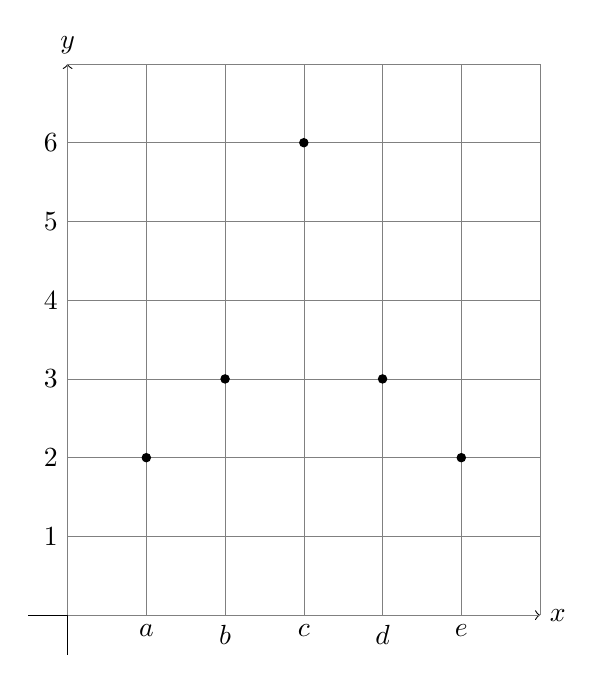
\begin{tikzpicture}[scale=1]
    % Ejes coordenados
    \draw[->] (-0.5, 0) -- (6, 0) node[right] {$x$};
    \draw[->] (0, -0.5) -- (0, 7) node[above] {$y$};

    % Cuadrícula
    \draw[step=1,gray,very thin] (0, 0) grid (6, 7);

    % Marcas del eje X
    \foreach \x/\label in {1/a, 2/b, 3/c, 4/d, 5/e} {
      \node[below] at (\x, 0) {$\label$};
    }

    % Marcas del eje Y
    \foreach \x in {1,...,6} {
      \node[left] at (0, \x) {$\x$};
    }

    % Puntos
    \filldraw (1, 2) circle (1.5pt);
    \filldraw (2, 3) circle (1.5pt);
    \filldraw (3, 6) circle (1.5pt);
    \filldraw (4, 3) circle (1.5pt);
    \filldraw (5, 2) circle (1.5pt);

  \end{tikzpicture}
  }
  \caption{Grafo de la aplicación $f$.}%
  \label{fig:interseccion-rectas}
\end{figure}

Al representar la aplicación $f$ en el conjunto producto $A \times B$ se
construye el grafo de la aplicación contenido en la
figura~\ref{fig:interseccion-rectas}.

Dado el grafo de una función $\{(x, f(x))\}$, se denomina
\emph{representación gráfica} de la función $f$ a la representación del
grafo en el conjunto producto correspondiente.

Ejemplo. Aplicación constante. Una aplicación $f: A \longrightarrow B$ se
dice \emph{constante} si y solo si la imagen de cada elemento de $A$ es
siempre el mismo elemento de $B$. Es decir,

$$ f: A \longrightarrow B \text{ es constante} \iff \forall x, x' \in A,
f(x) = f(x') $$

Ejemplo. Una relación de equivalencia $\erel$ definida sobre un conjunto $A$
permite definir la aplicación $p$ que asigna a cada elemento su clase de
equivalencia:

$$
  \begin{array}{llll}
    p:  & A   &\longrightarrow  & A/\erel \\
        & x   &\longmapsto      & p(x) = [x]
  \end{array}
$$

\noindent Esta aplicación se denomina \emph{proyección canónica} del
conjunto $A$ en el conjunto cociente.

Ejemplo. Una aplicación $f: A \longrightarrow B$ permite definir la
siguiente relación de equivalencia $\erel_f$ en $A$:

$$ x \erel_f y \iff f(x) = f(y) $$

Podemos por un lado considerar la proyección canónica $p$ del ejemplo
anterior y también considerar la aplicación $\tilde{f}$ que asigna a cada
clase de equivalencia la imagen mediante $f$ de uno cualquiera de sus
representantes:

$$
  \begin{array}{llll}
    \tilde{f}:  & A/\erel_f & \longrightarrow & B \\
                & [x]       & \longmapsto     & \tilde{f}([x]) = f(x)
  \end{array}
$$

La definición de la aplicación $\tilde{f}$ es consistente: no depende del
representante de la clase de equivalencia puesto que, si $[x] = [x']$,
entonces $x \erel_f x'$, es decir $f(x) = f(x')$.

Ejemplo. Aplicación identidad. Es la aplicación $I_A: A \longrightarrow A$
tal que la imagen de cada elemento de $A$ es el propio elemento. También
suele emplearse la notación $1_A$ o $\text{Id}_A$.

$$
  \begin{array}{llll}
    I_A:  & A & \longrightarrow & A \\
          & x & \longmapsto     & I_A(x) = x
  \end{array}
$$

\noindent Un caso particular de aplicación identidad sería en la que $A =
\rset$. Su representación gráfica es la recta $y = x$; es decir, la recta
diagonal del tercer y primer cuadrante.

Observación. Como una aplicación $f: A \longrightarrow B$ es una relación,
$f \subseteq A \times B$, entonces existe la relación inversa $f^{-1}
\subseteq B \times A$, definida por:

$$ f^{-1} = \{(y, x) \in B \times A \st f(x) = y\} = \{(f(x), x) \st x \in
A\} $$

En general, la relación inversa $f^{-1}$ correspondiente a una aplicación
$f$ no tiene por qué ser una aplicación. Así, se puede dar perfectamente
que, en $f$, algún elemento del conjunto final $B$ no sea imagen de ningún
elemento del conjunto origen o que haya dos elementos distintos del conjunto
original de $f$ con la misma imagen.

Ejemplo. El conjunto

$$ \{(x, y) \in \rset^2 \st x^2 - y = 0\} = \{(x, x^2) \st x \in \rset\} $$

\noindent es una aplicación $f$ de $\rset$ en $\rset$, definida como $f(x) =
x^2$, pero la relación $f^{-1}$ no es una aplicación, ya que, por ejemplo,
$f^{-1}(4) = \{{-2}, 2\}$.

\begin{figure}
  \centering
  \foreignlanguage{english}{
  \begin{tikzpicture}[scale=1]
    % Ejes cartesianos
    \draw[->] (-3, 0) -- (3, 0) node[below] {$x$};
    \draw[->] (0, -1) -- (0, 5) node[left] {$y$};

    % Dibujar las funciones de la parábola (superior e inferior)
    \draw[thick, domain=-2.2:2.2, samples=50] plot(\x, {pow(\x, 2)});

    % Puntos principales
    \filldraw (-2, 0) circle (1pt) node[below] {$x$};
    \filldraw (0, 4) circle (1pt) node[right] {$f(x)$};
    \filldraw (-2, 4) circle (1.5pt) node[anchor=south west] {$(x, x^2)$};

    % Líneas punteadas
    \draw[dashed] (-2, 0) -- (-2, 4) -- (0, 4);
  \end{tikzpicture}
  }
  \caption{Representación gráfica de la aplicación $f(x) = x^2$.}
  \label{fig:grafica_x_cuadrado}
\end{figure}

Igualdad de aplicaciones. Dos aplicaciones

\begin{align*}
  f&: A \longrightarrow B \\
  g&: A' \longrightarrow B' \\
\end{align*}

\noindent son iguales, $f = g$, si y solo si $A = A'$, $B = B'$ y, para todo
$x \in A$, $f(x) = g(x)$. Como ve, no basta que que se dé $f(x) = g(x)$.
Esta sutileza puede hacerle caer en errores. Así, cuando se da una función
por comprensión, a menudo se indica una expresión de la imagen de un
elemento genérico, por ejemplo, $f(x) = x^2$, pero no siempre se indica el
conjunto inicial o el conjunto final. En realidad, esto no debería hacerse,
puesto que las funciones

\begin{center}
\begin{minipage}[t]{.45\textwidth}
  \centering
  $$
    \begin{array}{llll}
      g:  & [0, \infty) & \longrightarrow & \rset \\
          & x           & \longmapsto     & g(x) = x^2
    \end{array}
  $$
\end{minipage}
\begin{minipage}[t]{.45\textwidth}
  \centering
  $$
    \begin{array}{llll}
      f:  & \rset & \longrightarrow & \rset \\
          & x     & \longmapsto     & f(x) = x^2
    \end{array}
  $$
\end{minipage}
\end{center}

\noindent son distintas, como puede comprobarse en las
figuras~\ref{fig:restriccion-dominio-1} y~\ref{fig:restricción-dominio-2}.
La diferencia se da, en este caso, únicamente en el dominio. De hecho, como
el conjunto inicial de $g$ está contenido en el conjunto inicial de $f$, y
sobre la parte común a ambos las funciones coinciden, se dice que $g$ es la
\emph{restricción} de $f$ a $[0, x)$ o que $f$ es una \emph{extensión} de
$g$ a $\rset$.

% TODO Quizás, quitarla y hacer la referencia a la de un ejercicio anterior.

\begin{figure}
  \centering
  \foreignlanguage{english}{
  \begin{tikzpicture}[scale=1]
    % Ejes cartesianos
    \draw[->] (-3, 0) -- (3, 0) node[below] {$x$};
    \draw[->] (0, -1) -- (0, 5) node[left] {$y$};

    % Dibujar las funciones de la parábola (superior e inferior)
    \draw[thick, domain=-2.2:2.2, samples=50] plot(\x, {pow(\x, 2)});

    % Etiqueta f
    \node at (-2, 2.5) {$f$};
  \end{tikzpicture}
  }
  \caption{Representación gráfica de la aplicación $f(x)$.}%
  \label{fig:restriccion-dominio-1}
\end{figure}

\begin{figure}
  \centering
  \foreignlanguage{english}{
  \begin{tikzpicture}[scale=1]
    % Ejes cartesianos
    \draw[->] (-3, 0) -- (3, 0) node[below] {$x$};
    \draw[->] (0, -1) -- (0, 5) node[left] {$y$};

    % Dibujar las funciones de la parábola (superior e inferior)
    \draw[thick, domain=0:2.2, samples=50] plot(\x, {pow(\x, 2)});

    % Etiqueta g
    \node at (2, 2.5) {$g$};
  \end{tikzpicture}
  }
  \caption{Restricción del dominio de la función $f$.}%
  \label{fig:restricción-dominio-2}
\end{figure}

Aun así, en la práctica es bastante común que uno se salte la especificación
del dominio de una función. Se trata de información elidida que el lector
deberá saber interpretar, según el contexto. La regla a seguir es considerar
el dominio de esta como el mayor conjunto donde la expresión de la imagen
posea sentido. A este conjunto se le llama \emph{campo de existencia} o
\emph{dominio de definición}. En el caso particular del ejemplo, se tiene
que $\text{Dom}(f) = \rset$.

Definición. Composición de aplicaciones. Dadas dos aplicaciones

\begin{align*}
  f&: A \longrightarrow B \\
  g&: B \longrightarrow C \\
\end{align*}

\noindent se define la composición de $f$ y $g$ como la aplicación $f: A
\longrightarrow C$ definida por $(g \circ f)(x) = g(f(x))$ para todo $x \in
A$.

Debe tener cuidado con la notación, pues existen textos en los que se altera
el orden, es decir, para los que $(g \circ f)(x) = f(g(x))$.

Muchas veces, como esta notación parece algo sobrecargada, si no hay lugar a
confusión se prefiere prescindir de los paréntesis y usar $g \circ f(x)$ en
lugar de $(g \circ f)(x)$.

El diagrama básico de la composición de funciones sería como el de una
función pero haciéndolo bidimensional, en lugar de unidimensional. Para los
datos de esta explicación, se tendría lo siguiente:

\begin{center}
\foreignlanguage{english}{
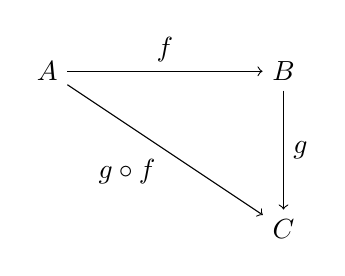
\begin{tikzpicture}[node distance=2cm, auto]
  % Nodos
  \node (A) at (0, 2) {$A$};
  \node (B) at (3, 2) {$B$};
  \node (C) at (3, 0) {$C$};

  % Flechas
  \draw[->] (A) -- (B) node[midway, above] {$f$};
  \draw[->] (B) -- (C) node[midway, right] {$g$};
  \draw[->] (A) -- (C) node[midway, below left] {$g \circ f$};
\end{tikzpicture}
}
\end{center}

En realidad, se podría dar una definición más amplia para la composición de
funciones. TKTK.

La composición de funciones no es conmutativa, es decir, en general, se
tiene que $f \circ g \neq g \circ f$. En primer lugar, si $f \in
\mathcal{F}(A, B)$ y $g \in \mathcal{F}(B, C)$, se tiene que $g \circ f \in
\mathcal{F}(A, C)$, pero la expresión $f \circ g$ carece en general de
sentido si $A \neq C$. Incluso en el caso de dos aplicaciones $f, g \in
\mathcal{F}(A)$, aun siendo las aplicaciones $g \circ f$ y $f \circ g$ ambas
elementos de $\mathcal{F}(A)$, en general, estas composiciones son
aplicaciones distintas, es decir, tal y como acabamos de comentar, la
composición de aplicaciones no cumple la propiedad conmutativa en
$\mathcal{F}(A)$, como puede comprobarse en el ejemplo TKTK.

Ejemplo. Sean las aplicaciones constantes

\begin{center}
\begin{minipage}[t]{.45\textwidth}
  \centering
  $$
    \begin{array}{llll}
      f:  & A & \longrightarrow & A \\
          & x & \longmapsto     & f(x) = a
    \end{array}
  $$
\end{minipage}
\begin{minipage}[t]{.45\textwidth}
  \centering
  $$
    \begin{array}{llll}
      g:  & A & \longrightarrow & A \\
          & x & \longmapsto     & g(x) = b
    \end{array}
  $$
\end{minipage}
\end{center}

\noindent siendo $a \neq b$. Para todo $x \in A$ se cumple lo siguiente:

\begin{align*}
  g \circ f(x) &= g(f(x)) = g(a) = b \\
  f \circ g(x) &= f(g(x)) = f(b) = a
\end{align*}


Propiedades.

Propiedad asociativa. Dadas tres aplicaciones $f \in \mathcal{F}(A, B)$, $g
\in \mathcal{F}(B, C)$ y $h \in \mathcal{F}(C, D)$, entonces

$$ (h \circ g) \circ f = h \circ (g \circ f). $$

\noindent En efecto:

$$ [h \circ (g \circ f)](x) = h((g \circ f)(x)) = h(g(f(x))) $$

\noindent y, por otro lado,

$$ [(h \circ g) \circ f](x) = (h \circ g)(f(x)) = h(g(f(x))), \ \forall x
\in A. $$

\noindent Esta propiedad permite escribir la composición de más de dos
aplicaciones sin tener que utilizar los paréntesis, por ejemplo, $h \circ g
\circ f$.

Propiedad. Dada una aplicación $f \in \mathcal{F}(A, B)$, entonces

\begin{center}
\begin{tabular}{lr}
  $f \circ I_a = f$
    & $I_b \circ f = f$
\end{tabular}
\end{center}

Son fáciles de demostrar. Advierta que $I_A \circ f$ en general no tiene
sentido, pues llegamos al punto en el que $(I_A \circ f)(x) = I_A(f(x))$,
pero $f(x) \in B$, con lo que puede que $I_A$ no sepa cómo operar a ese
argumento. Análogamente, para $f \circ I_B$.

Observación. Al restringir la composición de aplicaciones al conjunto de
aplicaciones $\mathcal{F}(A)$, entonces la composición es una operación
interna asociativa y con elemento neutro. Estos conceptos se verán en el
capítulo siguiente. Las notaciones $f^2$, $f^3$, \ldots, $f^n$ se utilizan
para indicar las composiciones

$$ f \circ f, f \circ f \circ f, \ldots, \overbrace{f \circ f \circ \cdots
\circ f}^{n\ \text{veces}} $$

Ejemplo. Sucesiones (\emph{sequences}) de elementos de un conjunto. Se
denomina \emph{sucesión} de elementos de un conjunto $A$ a una aplicación
cuyo conjunto inicial es el conjunto $\nset$ o $\nset^*$, es decir,
cualquier elemento $f \in \mathcal{F}(\nset, A)$ o $f \in
\mathcal{F}(\nset^*, A)$. Por ejemplo, una sucesión de números naturales $f
\in \mathcal{F}(\nset, \nset)$ definida por la expresión $f(n) = n^2, \
\forall n \in \nset$; la sucesión de los cuadrados de cada número natural.

Frecuentemente, la sucesión $f$ se presenta como una lista ilimitada de
números

$$ a_0, a_1, a_2, a_3, \ldots, a_n, \ldots $$

\noindent que son las imágenes de la lista de números naturales

$$ f(0), f(1), f(2), f(3), \ldots, f(n), \ldots $$

\noindent y al término $n$-ésimo, $f(n)$ o $a_n$, se le denomina
\emph{término general} de la sucesión. En el ejemplo anterior, la sucesión
es $0, 1, 4, 9, 16, \ldots, n^2, \ldots$.

Ejemplo. Función característica de un conjunto. Dado un subconjunto $A
\subseteq U$, se llama \emph{función característica} de $A$, y se denota por
$\chi_A$, a la función $\chi_A: U \longrightarrow \rset$ definida de la
forma:

$$
  \chi_A(x) =
  \begin{cases}
    1 & \text{si } x \in A, \\
    0 & \text{si } x \notin A.
  \end{cases}
$$

A continuación, destacamos algunas aplicaciones que poseen alguna
característica de interés en el conjunto de aplicaciones $\mathcal{F}(A,
B)$.

Definicón. Aplicación sobreyectiva o sobreyección. Es una aplicación tal que
cualquier elemento del conjunto final está relacionado con alguno del
conjunto inicial. Es decir, $f \in \mathcal{F}(A, B)$ tal que $\text{Im}(f)
= B$, o lo que es lo mismo:

$$ \forall y \in B, \ \exists x \in A \ \text{tal que} \ f(x) = y $$

Ejemplo. La representación gnifica de la figura~\ref{fig:grafica-x3}
correponde a la aplicación definida por $f(x) = x^3 - x$ para todo $x \in
\rset$. Se trata de una aplicación sobreyectiva de $\rset$ en $\rset$. Basta
observar que cualquier recta horizontal corta a la representación gráfica de
$f$ en al menos un punto. Para demostrar que es una aplicación sobreyectiva,
se comprueba que para todo $y \in \rset$ la ecuación en $x$, $x^3 - x = y$,
tiene al menos una solución. Esto se deduce del hecho de que toda ecuación
polinómica de grado impar tiene al menos una raíz en $\rset$.

\begin{figure}
  \centering
  \foreignlanguage{english}{
  \begin{tikzpicture}[scale=0.5]
    % Ejes cartesianos
    \draw[->] (-3, 0) -- (3, 0) node[below] {$x$};
    \draw[->] (0, -9) -- (0, 9) node[left] {$y$};

    % Dibujar las funciones de la parábola (superior e inferior)
    \draw[thick, domain=-2.2:2.2, samples=50] plot(\x, {pow(\x, 3) - \x});

    % Etiqueta f
    \node at (-2, 2.5) {$f$};
  \end{tikzpicture}
  }
  \caption{Representación gráfica de $f(x) = x^3 - x$.}%
  \label{fig:grafica-x3}
\end{figure}

En algunos textos, las aplicaciones sobreyectivas reciben otros nombres,
como \emph{aplicaciones suprayectivas}, \emph{aplicaciones exhaustivas},
etc. En inglés, también dicen \emph{onto} y otros nombres TKTK.

Definición. Aplicación inyectiva o inyección. Es una aplicación tal que no
hay dos elementos del conjunto inicial que tengan la misma imagen. Es decir,
$f \in \mathcal{F}(A, B)$ tal que

$$ \text{para todo } x, x' \in A, \text{ si } f(x) = f(x') \text{ entonces }
x = x' $$

\noindent O lo que es lo mismo,

$$ \text{para todo } x, x' \in A, \text{ si } x \neq x' \text{ entonces }
f(x) \neq f(x') $$

\noindent ya que esto es simplemente el condicional contrarrecíproco de la
anterior.

Ejemplo. La representación gráfica de la aplicación definida por $f(x) =
2^x$ para todo $x \in \rset$, que puede ver en la
figura~\ref{fig:grafica-2-elevado-x}, confirma que es una aplicación
inyectiva de $\rset$ en $\rset$. Basta observar que cualquier recta
horizontal corta a la representación gráfica de $f$ a lo sumo en un punto.
Para demostrar que es inyectiva, basta comprobar que si dos números $x$ y
$x'$ satisfacen la igualdad $f(x) = f(x')$, entonces $x = x'$. En este caso,

% TODO Hacerlo más compacto.

\begin{align*}
  f(x) &= f(x') \\
  2^x &= 2^{x'} \\
  \frac{2^x}{2^{x'}} &= \frac{2^{x'}}{2^{x'}} \\
  2^{x-x'} &= 1 \\
  \log_2 2^{x-x'} &= \log_2 1 \\
  (x - x')\log_2 2 &= 0 \\
  (x - x')\cdot 1 &= 0 \\
  x - x' &= 0 \\
  x &= x' \\
\end{align*}

\begin{figure}
  \centering
  \foreignlanguage{english}{
    \begin{tikzpicture}[scale=1]
    % Ejes cartesianos
    \draw[->] (-5, 0) -- (2, 0) node[below] {$x$};
    \draw[->] (0, -1) -- (0, 5) node[left] {$y$};

    % Dibujar las funciones de la parábola (superior e inferior)
    \draw[thick, domain=-5:2, samples=50] plot(\x, {pow(2, \x)});

    % Etiqueta f
    \node at (2, 2.5) {$f$};
  \end{tikzpicture}
  }
  \caption{Representación gráfica de $f(x) = 2^x$.}%
  \label{fig:grafica-2-elevado-x}
\end{figure}

Proposición. Dadas las aplicaciones $f \in \mathcal{F}(A, B)$, $g \in
\mathcal{F}(B, C)$ y $g \circ f \in \mathcal{F}(A, C)$, se tiene:

\begin{enumerate}
  \item Si $f$ y $g$ son sobreyectivas, entonces $g \circ f$ es
    sobreyectiva.
  \item Si $f$ y $g$ son inyectivas, entonces $g \circ f$ es inyectiva.
\end{enumerate}

Demostración.

La primera. Como $f(A) = B$, por ser $f$ sobreyectiva, y $g(B) = C$, por ser
$g$ sobreyectiva, se tiene que $g \circ f(A) = g(f(A)) = g(B) = C$. Luego la
composición es sobreyectiva.

La segunda. Dados $x, y \in A$ tales que $g \circ f(x) = g \circ f(y)$, o,
dicho de otra forma, $g(f(x)) = g(f(y))$. Como $g$ es inyectiva, se cumple
que $f(x) = f(y)$, y, por esto último, al ser $f$ inyectiva se tiene que $x
= y$. Luego la composición es una aplicación inyectiva.

Definición. Aplicación biyectiva. Una \emph{aplicación biyectiva} es una
aplicación que es sobreyectiva e inyectiva al mismo tiempo. Es decir, tal
que cada elemento del conjunto final está relacionado con un único elemento
del conjunto inicial. Es decir, una aplicación $f \in \mathcal{F}(A, B)$ tal
que

$$ \text{para cada } y \in B \text{ existe un único elemento } x \in A
\text{ tal que } f(x) = y. $$

Puede que vea que a una aplicación biyectiva la califican de
\emph{biyección}.

Ejemplo. Al observar la representación gráfica de la aplicación definida por
$f(x) = x^3$ para todo $x \in \rset$, como en la
figura~\ref{fig:grafica-x-cubo}, se comprueba que es una aplicación
biyectiva en de $\rset$ en $\rset$. Para demostrarlo, basta comprobar que
para cualquier $y \in \rset$, la ecuación $x^3 = y$ tiene una única solución
en $\rset$. En este caso, se tiene que $x = \sqrt[3]{y}$.

\begin{figure}
  \centering
  \foreignlanguage{english}{
  \begin{tikzpicture}[scale=0.5]
    % Ejes cartesianos
    \draw[->] (-3, 0) -- (3, 0) node[below] {$x$};
    \draw[->] (0, -9) -- (0, 9) node[left] {$y$};

    % Dibujar las funciones de la parábola (superior e inferior)
    \draw[thick, domain=-2:2, samples=50] plot(\x, {pow(\x, 3)});

    % Etiqueta f
    \node at (-2, 2.5) {$f$};
  \end{tikzpicture}
  }
  \caption{Representación gráfica de $f(x) = x^3$.}%
  \label{fig:grafica-x-cubo}
\end{figure}

Teorema. Caracterización de una aplicación biyectiva. Una aplicación $f \in
\mathcal{F}(A, B)$ es biyectiva si y solo si existe una aplicación $g \in
\mathcal{F}(B, A)$ tal que $f \circ g = I_B$ y $g \circ f = I_A$.

Demostración. Si $f$ es biyectiva, entonces la relación inversa $f^{-1}$ es
claramente una aplicación. Tomando $g = f^{-1}$ se cumple que $g \in
\mathcal{F}(B, A)$ y que $f \circ g = I_B$ y $g \circ f = I_A$.

Supongamos que existe una aplicación $g \in \mathcal{F}(B, A)$ tal que $f
\circ g = I_B$ y $g \circ f = I_A$. Para todo $y \in B$ existe al menos un
$x \in A$ tal que $f(x) = y$. Basta tomar $x = g(y)$. Si para algún $y \in
B$ existieran dos elementos $x, x' \in A$ tales que $f(x) = f(x') = y$,
entonces

$$ x = I_A(x) = g \circ f(x) = g(f(x)) = g(y) = g(f(x')) = g \circ f(x') =
I_A(x') = x'. $$

Luego para cada $y \in B$ existe un único $x \in A$ tal que $f(x) = y$.

Para cualquier aplicación biyectiva $f \in \mathcal{F}(A, B)$, la función $g
= f^{-1}$ del teorema anterior es única y se denomina \emph{aplicación
inversa} de la aplicación $f$. Además, la aplicación $f^{-1} \in
\mathcal{F}(B, A)$ es una aplicación biyectiva.

Teorema. Sean $f \in \mathcal{F}(A, B)$ y $g \in \mathcal{F}(B, C)$ dos
aplicaciones biyectivas, entonces la aplicación $g \circ f \in
\mathcal{F}(A, C)$ es biyectiva, y su inversa es:

$$ (g \circ f)^{-1} = f^{-1} \circ g^{-1}. $$

Demostración. Veamos que la aplicación $f^{-1} \circ g^{-1}$ cumple las
condiciones del teorema TKTK.

\begin{align*}
  (g \circ f) \circ (f^{-1} \circ g^{-1}) = g \circ (f \circ f^{-1}) \circ
    g^{-1} = g \circ I_B \circ g^{-1} = g \circ g^{-1} = I_C \\
  (f^{-1} \circ g^{-1}) \circ (g \circ f) = f^{-1} \circ (g^{-1} \circ g)
    \circ f = f^{-1} \circ I_B \circ f = f^{-1} \circ f = I_A \\
\end{align*}

Teorema. Sea una aplicación $f \in \mathcal{F}(A, B)$.

\begin{enumerate}
  \item $f$ es sobreyectiva si y solo si existe una aplicación $h \in
    \mathcal{F}(B, A)$ tal que $f \circ h = I_B$.
  \item $f$ es inyectiva si y solo si existe una aplicación $g \in
    \mathcal{F}(B, A)$ tal que $g \circ f = I_A$.
\end{enumerate}

Demostración. Veamos la equivalencia de ambos apartados mostrando las dos
implicaciones.

Para la primera. Si $f$ es sobreyectiva, entonces $\text{Im}(f) = B$. En
consecuencia, para todo $y \in \text{Im}(f)$, el conjunto $f^{-1}(\{y\})$ es
un conjunto no vacío. Sea $c_y$ un elemento de $f^{-1}(\{y\})$; por tanto,
$f(c_y) = y$. Se define:

$$
  \begin{array}{llll}
    h:  & B & \longrightarrow & A \\
        & y & \longmapsto     & h(y) = c_y \\
  \end{array}
$$

Así, pues, $f \circ h(y) = f(h(y)) = f(c_y) = y$, es decir, $f \circ h =
I_B$.

Recíprocamente, si existe la aplicación $h \in \mathcal{F}(B, A)$ tal que $f
\circ h = I_B$, entonces para cada $y \in B$ se tiene que $f(h(y)) = y$.
Luego $y \in \text{Im}(f)$ y, por tanto, $B \subseteq \text{Im}(f)$. Así,
pues, $f$ es sobreyectiva.

Para la segunda. Si $f$ es inyectiva, entonces para todo $y \in
\text{Im}(f)$ el conjunto $f^{-1}(y)$ es un conjunto unitario y denotando
por $a_y$ al único elemento de $f^{-1}(y)$ se cumple en particular que
$a_{f(x)} = x$. Sea un elemento $x_0 \in A$ fijo, se define

$$
  \begin{array}{llll}
    g:  & B & \longrightarrow & A \\
        & y & \longmapsto     & g(y) =
          \begin{cases}
            a_y & \text{si } y \in \text{Im}(f) \\
            x_0 & \text{si } y \notin \text{Im}(f)
          \end{cases}
        \\
  \end{array}
$$

Así pues, $g \circ f(x) = g(f(x)) = a_f(x) = x$ para cualquier $x \in A$.

Recíprocamente, si existe la aplicación $g \in \mathcal{F}(B, A)$ tal que $g
\circ f = I_A$, supuesto que existen $x_1$ y $x_2$ tales que $f(x_1) =
f(x_2)$, entonces

$$ x_1 = (g \circ f)(x_1) = g(f(x_1)) = g(f(x_2)) = (g \circ f)(x_2) = x_2
$$

\noindent Luego $f$ es inyectiva.

Nota. Si $f$ es sobreyectiva, la aplicación $h$ que se define en el primer
caso es inyectiva. Análogamente si $f$ es inyectiva, la aplicación $g$ que
se define en el segundo caso es sobreyectiva.

Observación. Como consecuencia del teorema TKTK, se tiene que si $f \in
\mathcal{F}(A, B)$ es una aplicación inyectiva, entonces la aplicación
$\hat{f} \in \mathcal{F}(A, f(A))$ que coincide con $f$ sobre $A$ y que
usualmente se denomina $f$, es una biyyección. Es decir, una aplicación
inyectiva de $A$ a $B$ da lugar a una aplicación biyectiva de $A$ al
conjunto imagen $\text{Im}(f) = f(A)$.





\subsection{Factorización canónica de una aplicación}

Vimos en el ejemplo TKTK cómo una aplicación $f: A \to B$ permite definir
una relación de equivalencia $\erel_f$ en el conjunto $A$ mediante:

$$ x \erel_f x' \quad \text{si y solo si} \quad f(x) = f(x') $$

\noindent y que esta a su vez permite definir una aplicación:

$$
  \begin{array}{llll}
    \tilde{f}:  & A/\erel_f & \longrightarrow & B \\
                & [x]       & \longmapsto     & \tilde{f}([x]) = f(x) \\
  \end{array}
$$

En el ejemplo TKTK, definimos la proyección canónica

$$
  \begin{array}{llll}
    p:  & A & \longrightarrow & A/\erel_f \\
        & x & \longmapsto     & p(x) = [x] \\
  \end{array}
$$

\noindent que por la definición de \emph{conjunto cociente} es una
aplicación sobreyectiva. Consideremos el siguiente diagrama.

\begin{center}
\foreignlanguage{english}{
\begin{tikzpicture}[node distance=2cm, auto]
  % Nodos
  \node (A) at (0, 3) {$A$};
  \node (B) at (3, 3) {$B$};
  \node (E) at (0, 0) {$A/\erel_f$};

  % Flechas
  \draw[->] (A) -- (B) node[midway, above] {$f$};
  \draw[->] (A) -- (E) node[midway, right] {$p$};
  \draw[->] (E) -- (B) node[midway, above left] {$\tilde{f}$};
\end{tikzpicture}
}
\end{center}

Se tiene $f = \tilde{f} \circ p$, pues para todo $x \in A$,

$$ \tilde{f} \circ p(x) = \tilde{f}(p(x)) = \tilde{f}([x]) = f(x) $$

Vamos a introducir en el diagrama anterior el conjunto imagen $f(A)
\subseteq B$, utilizando la aplicación

$$
  \begin{array}{llll}
    i:  & f(A)  & \longrightarrow & B \\
        & y     & \longmapsto     & i(y) = y \\
  \end{array}
$$

\noindent que es inyectiva y se denomina \emph{inyección canónica} o
\emph{aplicación inclusión}. Si consideramos además la aplicación

$$
  \begin{array}{llll}
    b:  & A/\erel_f & \longrightarrow & f(A) \\
        & [x]       & \longmapsto     & b([x]) = f(x) \\
  \end{array}
$$

\noindent entonces $b$ es una aplicación biyectiva. En efecto, sean $[x],
[x'] \in A/\erel_f$ arbitrarios. Si $b([x]) = b([x'])$ entonces $f(x) =
f(x')$, o, equivalentemente, $x \erel_f x'$. En consecuencia, $[x] = [x']$.
Por tanto, la aplicación $b$ es inyectiva.

Sea $y \in f(A)$ arbitrario. Existe $x \in A$ tal que $f(x) = y$. En
consecuencia, $b([x]) = y$. Como $[x] \in A/\erel_f$, se deduce que la
aplicación $b$ es sobreyectiva.

Finalmente, observemos que para todo $x \in A$ se cumple:

$$ (i \circ b \circ p)(x) = i \big(b(p(x))\big) = i\big(b([x])\big) =
i(f(x)) = f(x) $$

En definitiva, la descomposición canónica de la aplicación $f$ es:

\begin{center}
\foreignlanguage{english}{
\begin{tikzpicture}[node distance=2cm, auto]
  % Nodos
  \node (A) at (0, 3) {$A$};
  \node (B) at (3, 3) {$B$};
  \node (E) at (0, 0) {$A/\erel_f$};
  \node (F) at (3, 0) {$f(A)$};

  % Flechas
  \draw[->] (A) -- (B) node[midway, below] {$f$};
  \draw[->] (A) -- (E) node[midway, right] {$p$};
  \draw[->] (E) -- (F) node[midway, above] {$b$};
  \draw[->] (F) -- (B) node[midway, left] {$i$};
\end{tikzpicture}
}
\end{center}

\noindent donde:

$$ f = i \circ b \circ p $$

\noindent siendo

\begin{center}
  \begin{tabular}{ll}
    $p$ & proyección canónica de $A$ en $A/\erel_f$ \\
    $b$ & biyección canónica de $A/\erel_f$ en $f(A)$ \\
    $i$ & inyección canónica de $f(A)$ en $B$ \\
  \end{tabular}
\end{center}

Ejemplo. Veamos la descomposición canónica de la función

$$
  \begin{array}{llll}
    f:  & \rset & \longrightarrow & \rset \\
        & x     & \longmapsto     & f(x) = \sin(x) \\
  \end{array}
$$

En este caso, $f(\rset) = [{-1}, 1]$ y la relación de equivalencia que
define $f$ es

$$ x \erel_f x' \iff \sin(x) = \sin(x') $$

\noindent y, en consecuencia,

$$ [x] = \{x' \in \rset \st x' = x + 2\pi k \ \text{o} \ x' = \pi x + 2 \pi
k, \ \text{con} \ k \in \zset\} $$

Obsérvese que siempre existe un único representante de lcada clase en el
intervalo $[{-\pi/2}, \pi/2]$.

\begin{center}
\foreignlanguage{english}{
\begin{tikzpicture}[node distance=2cm, auto]
  % Nodos
  \node (A) at (0, 3) {$\rset$};
  \node (B) at (3, 3) {$\rset$};
  \node (E) at (0, 0) {$\rset/\erel_f$};
  \node (F) at (3, 0) {$[{-1}, 1]$};

  % Flechas
  \draw[->] (A) -- (B) node[midway, below] {$f$};
  \draw[->] (A) -- (E) node[midway, right] {$p$};
  \draw[->] (E) -- (F) node[midway, above] {$b$};
  \draw[->] (F) -- (B) node[midway, left] {$i$};
\end{tikzpicture}
}
\end{center}

\noindent donde:

$$ f = i \circ b \circ p $$

\noindent siendo

\begin{center}
  \begin{tabular}{ll}
    $p$ & proyección canónica de $\rset$ en $\rset/\erel_f$ \\
    $b$ & biyección canónica de $\rset/\erel_f$ en $[{-1}, 1]$ \\
    $i$ & inyección canónica de $[{-1}, 1]$ en $\rset$ \\
  \end{tabular}
\end{center}











